% \iffalse
\let\negmedspace\undefined
\let\negthickspace\undefined
\documentclass[journal,12pt,twocolumn]{IEEEtran}
\usepackage{amssymb}
\usepackage{cite}
\usepackage{amsmath,amssymb,amsfonts,amsthm}
\usepackage{algorithmic}
\usepackage{graphicx}
\usepackage{textcomp}
\usepackage{xcolor}
\usepackage{txfonts}
\usepackage{listings}
\usepackage{enumitem}
\usepackage{mathtools}
\usepackage{gensymb}
\usepackage{comment}
\usepackage[breaklinks=true]{hyperref}
\usepackage{tkz-euclide} 
\usepackage{listings}
\usepackage{gvv}                                        
\def\inputGnumericTable{}                                 
\usepackage[latin1]{inputenc}                                
\usepackage{color}                                            
\usepackage{array}                                            
\usepackage{longtable}                                       
\usepackage{calc}                                             
\usepackage{multirow}                                         
\usepackage{hhline}                                           
\usepackage{ifthen}                                           
\usepackage{lscape}
\usepackage{pgfplots}
\newtheorem{theorem}{Theorem}[section]
\newtheorem{problem}{Problem}
\newtheorem{proposition}{Proposition}[section]
\newtheorem{lemma}{Lemma}[section]
\newtheorem{corollary}[theorem]{Corollary}
\newtheorem{example}{Example}[section]
\newtheorem{definition}[problem]{Definition}
\newcommand{\BEQA}{\begin{eqnarray}}
\newcommand{\EEQA}{\end{eqnarray}}
\newcommand{\define}{\stackrel{\triangle}{=}}
\theoremstyle{remark}
\newtheorem{rem}{Remark}
\begin{document}

\bibliographystyle{IEEEtran}
\vspace{3cm}

\title{GATE.2021.EE.46}
\author{EE22BTECH11004 - Allu Lohith}

\maketitle
\newpage
\bigskip

\renewcommand{\thefigure}{\theenumi}
\renewcommand{\thetable}{\theenumi}

Consider a closed-loop system as shown, $$G_p\brak s= \frac{14.4}{s\brak{1+0.1s}}$$ is the plant transfer function and $G_c\brak s=1$ is the compensator. For a unit-step input, the output response has damped oscillations. The damped natural frequency is $\underline{\hspace{2cm}}$
$rad/s$. (Round off to 2 decimal places.)

\begin{figure}[h]
    \centering  
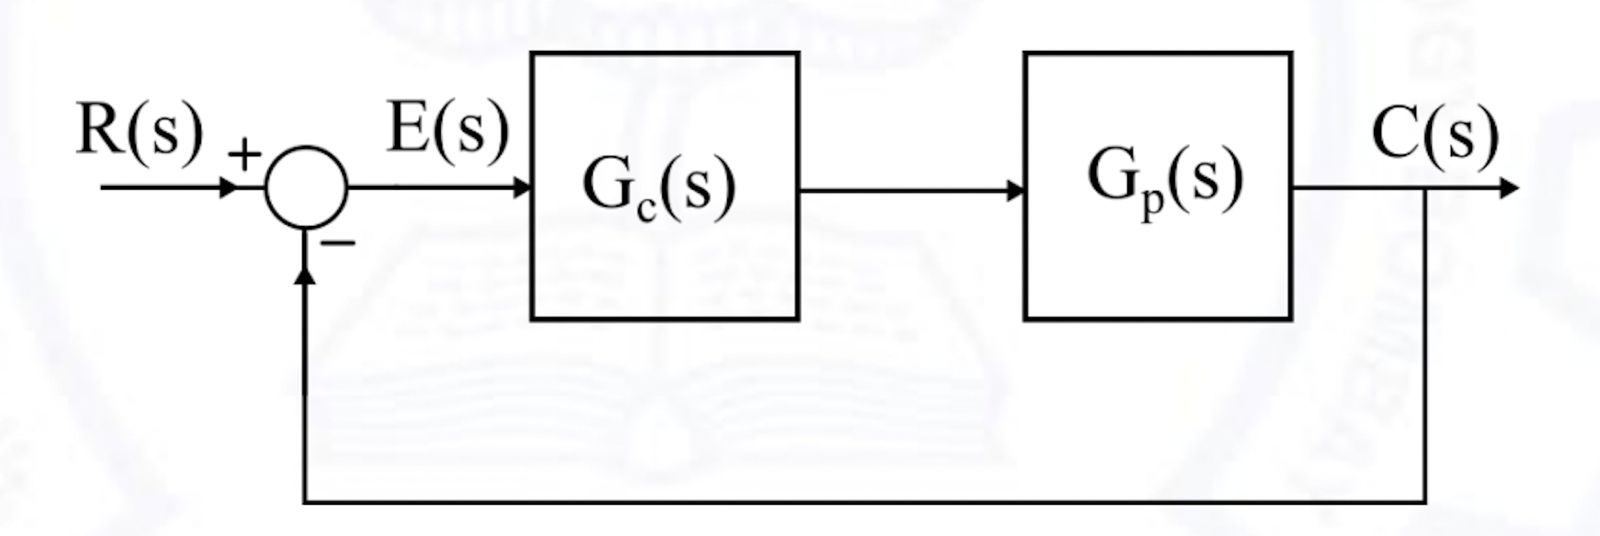
\includegraphics[width=\columnwidth]{figs/dia.png}
    \label{fig:}
\end{figure}
\solution 
\begin{table}[h!]
\centering
\renewcommand{\arraystretch}{2}
\begin{tabular}{|p{2cm}|p{3cm}|p{2cm}|}
\hline 
\setlength{\tabcolsep}{1pt}
\textbf{Parameter}  &\textbf{Description} &\textbf{Value} \\
\hline
$G_n\brak s$ & Plant transfer function & $\dfrac{14.4}{s\brak{1+0.1s}}$ \\
\hline
$G_c\brak{s}$ &Transfer function of the compensator  & 1 \\
\hline
$\omega_n$ & Damped natural frequency& - \\
\hline
$T$& Overall tranfer function & $\dfrac{C}{R}$\\
\hline
\end{tabular}

\vspace{0.5cm}
\caption{\normalsize Parameters}
\end{table}
As we know that:
\begin{align}
E&=R_c-C_c\\
EG_cG_p&=C
\end{align}
So,
\begin{align}
E &= \frac{Cs\brak{1+0.1s}}{14.4}\\
\frac{Cs\brak{1+0.1s}}{14.4} &=R-C\\
R &=C\brak{\frac{s\brak{1+0.1s}}{14.4}+1}\\
\frac{C}{R} &= \frac{14.4}{0.1s^2+s+14.4}
\end{align}
The characteristic equation is $0.1s^2+s+14.4$ which is of the form $s^2 + 2\zeta\omega_n s + \omega_n^2$, So 
\begin{align}
    \omega_n^2&=144\\
    \omega_n&= 12rad/s
\end{align}

\begin{figure}[h]
    \centering  

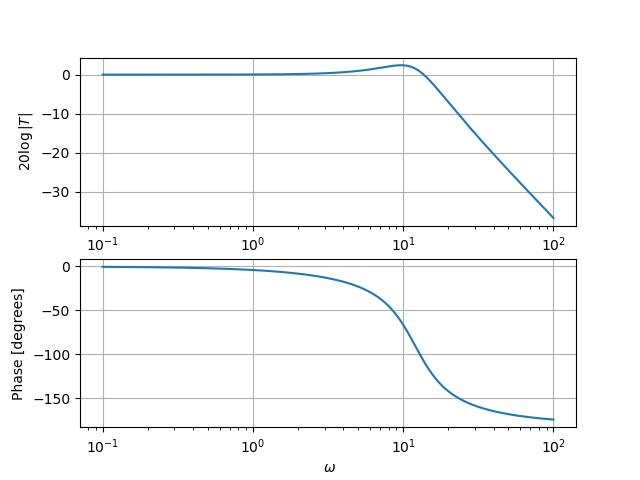
\includegraphics[width=\columnwidth]{figs/plot.png}

    \centering
    \caption{Bode Plot - Magnitude and Phase Response}

    \label{fig:}
\end{figure}

\end{document}
